\section{Map 映射}

Map 接口已经在前文说明过,不再介绍。Map 的底层实现逻辑是容器中最复杂,但由于 Set 容器需要依赖 Map 实现,所以必须先讲 Map。

\begin{center}
    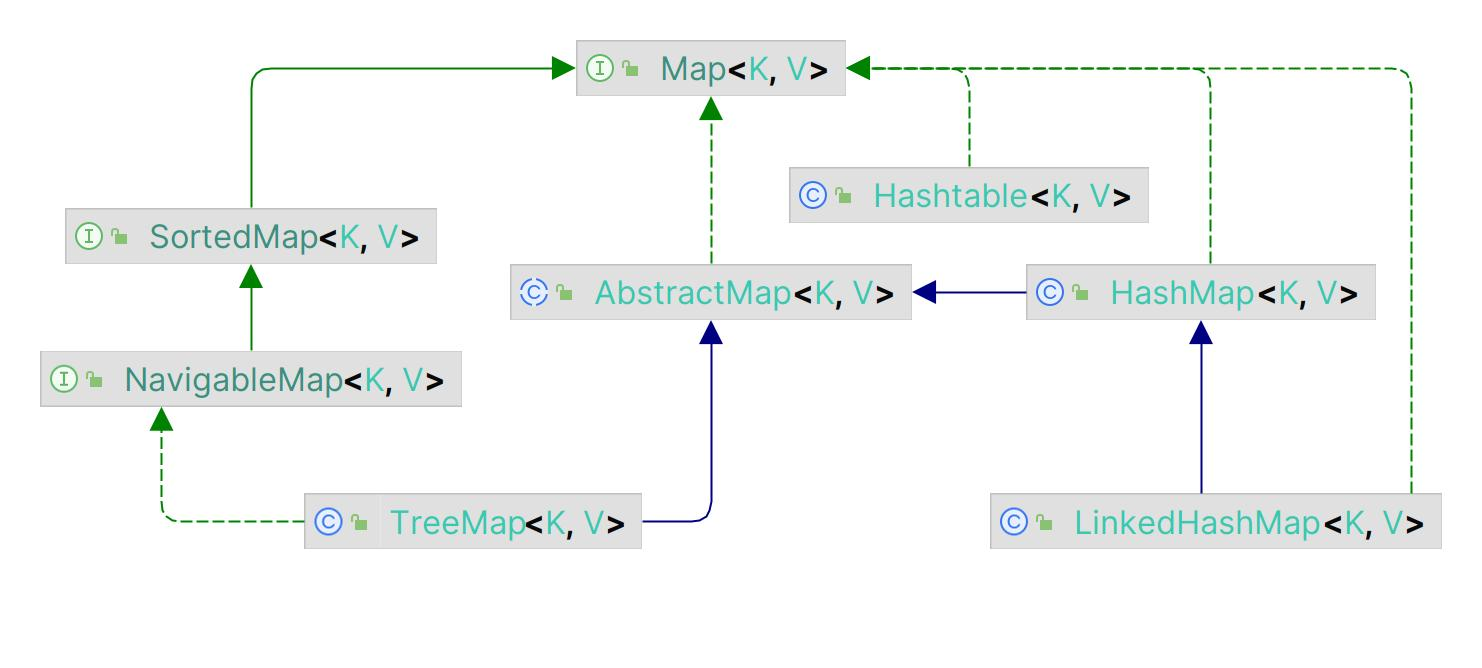
\includegraphics[width=0.8\linewidth]{../../imgs/Map.jpg}
\end{center}

\subsection{HashTable}

Hashtable 是 HashMap 的古早实现,现在已经不推荐使用 Hashtable 而应该使用 HashMap,但 Hashtable 相对较简单,而且和 Vector 与 ArrayList 的关系类似,Hashtable 是线程安全的,这章只利用 Hashtable 作为切入口,简单入门哈希表结构,不做详细说明。

我们知道,底层数据结构的物理存储结构只有两种:顺序存储结构与链式存储结构。List 的 ArrayList 与 LinkedList 底层实现就对应了这两种储存结构。其他所有的数据结构都是基于这两种物理组织形式。

\begin{itemize}
    \item 顺序存储:直接或间接采用数组实现,需要连续的存储单元存储数据,可以快速查询,但插入删除操作较慢。
    \item 线性存储:一般采用链表实现,插删操作非常快,查找则需要遍历。
\end{itemize}

哈希表的底层实现就是这两种存储结构的结合,通过数组快速定位,通过链表解决哈希冲突:

\begin{Java}
public class Hashtable<K,V> extends Dictionary<K,V> implements Map<K,V>, Cloneable, java.io.Serializable
\end{Java}

\subsubsection{Dictionary 字典}

可以看到,Hashtable 直接继承自 Dictionary,熟悉 Python 或者 Json 的读者对字典肯定不陌生,字典是所有实现了键值映射的类的抽象基类,他为我们提供了一些基础方法(全是抽象的)。

\begin{itemize}
    \item int size(): 获取大小。
    \item boolean isEmpty(): 判断是否为空。
    \item Enumeration<K> keys(): 获取所有键。
    \item Enumeration<K> elements(): 获取所有值。
    \item V get(Object key): 通过键获取值。
    \item V put(K key, V value): 插入键值对。
    \item V remove(Object key): 通过键删除键值对。
\end{itemize}

这些方法,Map 接口也基本都定义了,但 Dictionary 并不是 Map,它的抽象程度更高,同时没有 entry,更加``轻量化''。

比较关键的两个方法 keys(), elements() 返回的是 Enumeration 对象,Enumeration 是一个接口。

\begin{Java}
public interface Enumeration<E>
\end{Java}

Enumeration 定义了从一个数据结构得到连续数据的手段,它提供了两个主要方法:

\begin{itemize}
    \item boolean hasMoreElements(): 判断是否还有元素。
    \item E nextElement(): 获取下一个元素。
\end{itemize}

还有一个给了默认实现的方法,其实是将上面两个方法封装成迭代器:

\begin{Java}
default Iterator<E> asIterator() {
    return new Iterator<>() {
        @Override public boolean hasNext() {
            return hasMoreElements();
        }
        @Override public E next() {
            return nextElement();
        }
    };
}
\end{Java}

这些东西全都没实现,留给 Hashtable 完成。

\subsubsection{Entry 单向链表}

Entry 在 Map 和 Set 中经常使用,不同容器的 Entry 大同小异,下面看一下 Hashtable 的 Entry:

\begin{Java}
private static class Entry<K,V> implements Map.Entry<K,V>  
\end{Java}

Hashtable.Entry 实现了 Map.Entry 接口,Map.Entry 接口定义了对 Entry 的基本操作,包含一些 get,set,compare 方法。Hashtable.Entry 的方法也类似,但它的数据存储结构非常重要,它的重要成员与构造函数如下。

\begin{Java}
final int hash;
final K key;
V value;
Entry<K,V> next;
protected Entry(int hash, K key, V value, Entry<K,V> next) {
    ...
}
\end{Java}

可以看到,它包含了三个基本成员,hash 对应哈希值,key,value 为一组键值对,如果 hash 值相同(出现了哈希碰撞),则需要通过比较 key 进一步判断(不比较值肯定是因为值不好比较)。

此外,Entry 只有一个 Entry<K,V> next 用于获取下一个 Entry 对象,这说明 Entry 集合是单向链表的。

\subsubsection{哈希表存储原理}

理解哈希表实现原理之前先看一下最关键的 构造函数,put\footnote{为什么不叫 add,因为 Hashtable 不是顺序加入,且需要添加 K-V。} 与 get 方法。

\begin{Java}
public Hashtable() {
    this(11, 0.75f);
}

public Hashtable(int initialCapacity, float loadFactor) {
    if (initialCapacity < 0)
        throw new IllegalArgumentException("Illegal Capacity: "+
                                           initialCapacity);
    if (loadFactor <= 0 || Float.isNaN(loadFactor))
        throw new IllegalArgumentException("Illegal Load: "+loadFactor);
    if (initialCapacity==0)
        initialCapacity = 1;
    this.loadFactor = loadFactor;
    table = new Entry<?,?>[initialCapacity];
    threshold = (int)Math.min(initialCapacity * loadFactor, MAX_ARRAY_SIZE + 1);
}
\end{Java}

其中 loadFactor 是负载系数,用于降低哈希碰撞,具体作用在 HashMap 节中说明,initialCapacity 为初始化数组大小。

构造函数本质上初始化了三个值:

\begin{Java}
private float loadFactor;   // 负载系数
private transient Entry<?,?>[] table;   // 哈希表,用于存储核心数据
private int threshold;      // 用于判断是否要重新哈希
\end{Java}

最核心的,根据参数(默认为11),创建了一个指定大小的 Entry 数组。然后来看一下加入键值对后会发生的事:

\begin{Java}
public synchronized V put(K key, V value) {
    if (value == null) {
        throw new NullPointerException();
    }
    Entry<?,?> tab[] = table;
    int hash = key.hashCode();
    int index = (hash & 0x7FFFFFFF) % tab.length;
    @SuppressWarnings("unchecked")
    Entry<K,V> entry = (Entry<K,V>)tab[index];
    for(; entry != null ; entry = entry.next) {
        if ((entry.hash == hash) && entry.key.equals(key)) {
            V old = entry.value;
            entry.value = value;
            return old;
        }
    }
    addEntry(hash, key, value, index);
    return null;
}

private void addEntry(int hash, K key, V value, int index) {
    Entry<?,?> tab[] = table;
    if (count >= threshold) {
        // Rehash the table if the threshold is exceeded
        rehash();

        tab = table;
        hash = key.hashCode();
        index = (hash & 0x7FFFFFFF) % tab.length;
    }
    // Creates the new entry.
    @SuppressWarnings("unchecked")
    Entry<K,V> e = (Entry<K,V>) tab[index];
    tab[index] = new Entry<>(hash, key, value, e);
    count++;
    modCount++;
}
\end{Java}

其中 0x7FFFFFFF 是 32 位最大整数,hash 值与他进行与运算能保证结果必为正数,再取余计算出 index 值。然后加入到 table 数组对应的位置中,如果该位置已经有元素,比较 key 值,没有则放在 Entry 单向链表的尾部,有则改变。

为什么要单独 Entry<?,?> tab[] = table 拿一个 table 引用,多线程!

比较重要的,如果哈希表中元素过多,会对哈希表进行 rehash 操作,本质上是扩大 table 数组。

最后看一下 get 方法,逻辑和 put 类似,找到对应 index 和 key 值,取 value:

\begin{Java}
public synchronized V get(Object key) {
    Entry<?,?> tab[] = table;
    int hash = key.hashCode();
    int index = (hash & 0x7FFFFFFF) % tab.length;
    for (Entry<?,?> e = tab[index] ; e != null ; e = e.next) {
        if ((e.hash == hash) && e.key.equals(key)) {
            return (V)e.value;
        }
    }
    return null;
}
\end{Java}

最后用一张图解释哈希表的存储结构:

\begin{figure}[H]
    \small
    \centering
    \begin{tikzpicture}[scale = 1]
        \node (text) at (0,1.5) {(hash \& 0x7FFFFFFF) \% tab.length 计算出数组下标};
        \matrix [nodes = {minimum height=10mm, text width=1cm, align=center}] at (0,0.7)
        {
            \node (0) {0}; & \node (1) {1}; & \node (2) {2}; & \node(3) {3} ; & \node(4) {4}; & \node(5) {5}; & \node(6) {6}; & \node(7) {...}; & \node(10) {n};\\
        };
        \matrix [nodes = {draw, fill=blue!10, minimum height=10mm, text width=1cm, align=center}] at (0,0)
        {
            \node (0) {Entry}; & \node (1) {null}; & \node (2) {Entry}; & \node(3) {Entry} ; & \node(4) {Entry}; & \node(5) {Entry}; & \node(6) {Entry}; & \node(7) {...}; & \node(10) {Entry};\\
        };

        \matrix [nodes = {fill=red!10, minimum height=10mm, text width=1cm, align=center}] at (0,-1.5)
        {
            \node (0-1) {Entry}; & \node[fill=white] (1-1) {}; & \node (2-1) {Entry}; & \node[fill=white] (3-1) {}; & \node(4-1) {Entry}; & \node(5-1) {Entry}; & \node[fill=white] (6-1) {}; & \node[fill=white] (7-1) {}; & \node[fill=white] (10-1) {}; \\
        };
        \matrix [nodes = {fill=red!10, minimum height=10mm, text width=1cm, align=center}] at (0,-3)
        {
            \node[fill=white] (0-2) {}; & \node[fill=white] (1-2) {}; & \node (2-2) {Entry}; & \node[fill=white] (3-2) {}; & \node(4-2) {Entry}; & \node[fill=white] (5-2) {}; & \node[fill=white] (6-2) {}; & \node[fill=white] (7-2) {}; & \node[fill=white] (10-2) {}; \\
        };
        \matrix [nodes = {fill=red!10, minimum height=10mm, text width=1cm, align=center}] at (0,-4.5)
        {
            \node[fill=white] (0-3) {}; & \node[fill=white] (1-3) {}; & \node (2-3) {Entry}; & \node[fill=white] (3-3) {}; & \node[fill=white] (4-3) {}; & \node[fill=white] (5-3) {}; & \node[fill=white] (6-3) {}; & \node[fill=white] (7-3) {}; & \node[fill=white] (10-3) {}; \\
        };
        \draw [-Stealth] (0) -- (0-1);
        \draw [-Stealth] (2) -- (2-1);
        \draw [-Stealth] (2-1) -- (2-2);
        \draw [-Stealth] (2-2) -- (2-3);
        \draw [-Stealth] (4) -- (4-1);
        \draw [-Stealth] (4-1) -- (4-2);
        \draw [-Stealth] (5) -- (5-1);
    \end{tikzpicture}
    \caption{HashTable 存储结构}
    \label{fig:HashTable 存储结构}
\end{figure}

\subsection{HashMap}

\subsubsection{红黑树}

\fbox{
    \parbox{0.87\textwidth}{
        \begin{notice}
            这节主要介绍原理,不对具体算法做过多研究。红黑树是一个高度综合的数据结构,涉及到二叉树的平衡问题,染色问题。虽然不是看不懂的数据结构,但也属于看得懂中较难的层次,如果扩展开来从头讲,这一节将成为最长的一节。因此,本节只将最基础的理论,以及 Java 的具体实现。
        \end{notice}
    }
}

Hashtable 在查找时还存在一个问题:Entry 单链表很长怎么办,无论数组多长,只需要计算一次就可以得到下标值。但单链表不同,他需要每次取 key 值进行比较,如果单链表过长,查找的速度仍然很慢。HashMap 为了解决这个问题加入了新的数据结构: 红黑树。

红黑树是一种自平衡的二叉查找树,二叉查找树时满足以下三个特性的二叉树:
\begin{itemize}
    \item 若左子树非空,则左子树上所有节点的值都小于根节点的值;
    \item 若其右子树非空,则右子树上所有节点的值都大于根节点的值;
    \item 其左右子树都是一棵二叉查找树。
\end{itemize}

讲人话,如果画的标准,将所有节点映射向下到平面上,节点的值是从大到小排列的。

二叉查找树可以进行十分快速的插入,删除,查找操作,但是它存在一种极端情况,插入的数据是顺序递增或者递减的,这样二叉查找树会退化为单链表。为了解决这个问题,需要平衡二叉查找树。

平衡就是保持每个节点左子树和右子树高度差不超过1。但如果要满足平衡二叉树,在频繁插入和删除操作过程中,由于二叉树需要旋转保持平衡,非常消耗性能。权衡利弊,Java 选择了红黑树,而红黑树是一种接近平衡的二叉树。

红黑树是一个二叉搜索树,它在每个节点增加了一个存储位记录节点的颜色,可以是RED,也可以是BLACK(实际上用 boolean 标记,true 为 REA,false 为 BLACK)。它具有以下性质:

\begin{itemize}
    \item 根节点是 BLACK;
    \item 节点被标记为 RED 或 BLACK;
    \item 叶子节点都是 null 且为 BLACK,null节点的父节点在红黑树里不将其看作叶子节点;
    \item RED 节点的子节点和父节点都是 BLACK 节点(从根节点到叶子节点的所有路径上不能有 2 个连续的红色节点)。
    \item 从任一节点到叶子节点(null节点)的所有路径都包含相同数目的黑色节点。
\end{itemize}

在 Java 中红黑树节点的关键属性如下:

\begin{Java}
static final class TreeNode<K,V> extends LinkedHashMap.Entry<K,V> {
    TreeNode<K,V> parent;
    TreeNode<K,V> left;
    TreeNode<K,V> right;
    TreeNode<K,V> prev;
    boolean red;
}
\end{Java}

此外,还封装了如旋转,平衡,查找等操作,实际开发过程中,我们并不会用到这些操作。

\subsubsection{底层实现}

在 JDK8 之前,HashMap 采用的是链表哈希,和前面 Hashtable 原理一致。

首先看一下构造方法:

\begin{Java}
public HashMap() {
    this.loadFactor = DEFAULT_LOAD_FACTOR; // all other fields defaulted
}
\end{Java}

默认构造函数只指定了一个负载系数,这玩意在 HashMap 中实际起作用只有两句(resize 和 putMapEntries 方法中)同样的话:

\begin{Java}
float ft = ((float)s / loadFactor) + 1.0F;
int t = ((ft < (float)MAXIMUM_CAPACITY) ? (int)ft : MAXIMUM_CAPACITY);
if (t > threshold) threshold = tableSizeFor(t);
\end{Java}

其作用是决定哈希表数组的大小,loadFactor 越大,数组长度越小,空间利用率越高,哈希冲突发生可能性越高。一般的使用默认的 0.75 即可。

接下来看 put 方法:

\begin{Java}
public V put(K key, V value) {
    return putVal(hash(key), key, value, false, true);
}
\end{Java}

这个 putVal 方法很长,先看 hash 方法:

\begin{Java}
static final int hash(Object key) {
    int h;
    return (key == null) ? 0 : (h = key.hashCode()) ^ (h >>> 16);
}
\end{Java}

不同于 Hashtale 直接用 key.hashCode() 作为哈希值,HashMap 加了一步运算,这样的好处如下:
\begin{itemize}
    \item 右移16位是为了让高16位也参与运算,可以更好的均匀散列,减少碰撞。
    \item 异或运算是为了更好保留两组32位二进制数中各自的特征。
\end{itemize}

总而言之,这样一算,就更难发生哈希碰撞了。

下面看 putVal 方法(非常恐怖):

\begin{Java}
final V putVal(int hash, K key, V value, boolean onlyIfAbsent, boolean evict) {
    Node<K,V>[] tab; Node<K,V> p; int n, i;
    // 判断 table 表是否为空,为空则 resize 整一个
    if ((tab = table) == null || (n = tab.length) == 0)
        n = (tab = resize()).length;
    // 判断 table 表指定位置中元素是否为 null
    if ((p = tab[i = (n - 1) & hash]) == null)
        tab[i] = newNode(hash, key, value, null);   // null 则直接放 Node
    else {  // 不是 null 就麻烦了
        Node<K,V> e; K k;
        // 通过 hash 和 key 判断相同
        if (p.hash == hash && ((k = p.key) == key || (key != null && key.equals(k))))
            e = p;
        // 如果这个元素是 TreeNode 类型,放入红黑树
        else if (p instanceof TreeNode)
            e = ((TreeNode<K,V>)p).putTreeVal(this, tab, hash, key, value);
        // 向单链表添加数据
        else {
            for (int binCount = 0; ; ++binCount) {
                if ((e = p.next) == null) {
                    p.next = newNode(hash, key, value, null);
                    // 添加过程中发现单链表长度大于等于 8,转换为 红黑树
                    if (binCount >= TREEIFY_THRESHOLD - 1) // -1 for 1st
                        treeifyBin(tab, hash);
                    break;
                }
                if (e.hash == hash &&
                    ((k = e.key) == key || (key != null && key.equals(k))))
                    break;
                p = e;
            }
        }
        // null 特殊处理
        if (e != null) {
            V oldValue = e.value;
            if (!onlyIfAbsent || oldValue == null)
                e.value = value;
            afterNodeAccess(e);
            return oldValue;
        }
    }
    ++modCount;
    // 判断是否要扩容
    if (++size > threshold)
        resize();
    afterNodeInsertion(evict);
    return null;
}
\end{Java}

对比 Hashtable,put 方法变复杂的主要原因有如下:
\begin{itemize}
    \item 红黑树: 需要判断是插入链表还是插入红黑树,还是插入到链表后需要转换为红黑树。
    \item null: 不同于 Hashtable,HashMap 可以添加键为 null 的一个 Entry,以及值为 null 的多个节点。
\end{itemize}

对应的,remove 操作也变得十分复杂,但逻辑都类似。

\subsection{TreeMap}

TreeMap 是只是用红黑树存储的一种映射,他没有使用 hashCode 进行排序,默认使用自然序列(整数的升序,字符串的字母表排序)排列,可以通过 Comparator 接口指定排列方式。

\begin{Java}
public class TreeMap<K,V> extends AbstractMap<K,V> implements NavigableMap<K,V>, Cloneable, java.io.Serializable
\end{Java}

\begin{Java}
public TreeMap() {
    comparator = null;
}
\end{Java}

它实现了 NavigableMap 接口,该接口字面意思是可导航的,而 NavigableMap 接口又继承自 SortedMap 可以理解为是有序映射。

\begin{Java}
public interface NavigableMap<K,V> extends SortedMap<K,V>
public interface SortedMap<K,V> extends Map<K,V>
\end{Java}

SortedMap 包含以下几个常用方法:
\begin{itemize}
    \item SortedMap<K,V> subMap(K fromKey, K toKey): 获取键范围子映射。
    \item SortedMap<K,V> headMap(K toKey): 获取头部子映射,相当于 fromKey 为首个 key。
    \item SortedMap<K,V> tailMap(K fromKey): 获取尾部子映射,相当于 toKey 为最后一个 key。
    \item K firstKey() / lastKey(): 获取第一/最后一个 key。
\end{itemize}

NavigableMap 在 SortedMap 基础上增加了很多类似的新的方法,可以更灵活的返回 K,V,Entry 对象。

\subsection{LinkedHashMap}

如果说 TreeMap 是 HashMap - 数组, 那么 LinkedHashMap 就是 HashMap + 双向链表。LinkedHashMap 在不对HashMap做任何改变的基础上,给HashMap的任意两个节点间加了两条连线(before指针和after指针),使这些节点形成一个双向链表。

\begin{Java}
public class LinkedHashMap<K,V> extends HashMap<K,V> implements Map<K,V>
\end{Java}

在LinkedHashMapMap中,所有put进来的Entry都保存在HashMap中,但由于它又额外定义了一个以head为头结点的空的双向链表,因此对于每次put进来Entry还会将其插入到双向链表的尾部。

\begin{Java}
public LinkedHashMap() {
    super();
    accessOrder = false;
}
\end{Java}

构造方法增添了一个 accessOrder,默认为 false,表示按插入顺序遍历,设置为 true 表示按访问顺序遍历。按插入顺序遍历,这是和 TreeMap 在功能上最大的不同。

为了实现双向链表,LinkedHashMap 对 Node 增添了两个引用:

\begin{Java}
static class Entry<K,V> extends HashMap.Node<K,V> {
    Entry<K,V> before, after;
    Entry(int hash, K key, V value, Node<K,V> next) {
        super(hash, key, value, next);
    }
}
\end{Java}

类似 LinkedList,LinkedHashMap 也添加了头部和尾部节点:

\begin{Java}
transient LinkedHashMap.Entry<K,V> head;
transient LinkedHashMap.Entry<K,V> tail;
\end{Java}

具体实现逻辑不讲了,参考 LinkedList。

\newpage